%% PNAStwoS.tex
%% Sample file to use for PNAS articles prepared in LaTeX
%% For two column PNAS articles
%% Version1: Apr 15, 2008
%% Version2: Oct 04, 2013

%% BASIC CLASS FILE
\documentclass{pnastwo}

%% ADDITIONAL OPTIONAL STYLE FILES Font specification

%\usepackage{pnastwoF}
%\usepackage{cite}
\usepackage[numbers,round,sort,compress]{natbib}
\bibpunct{(}{)}{,}{n}{,}{,}  % https://xianblog.wordpress.com/tag/natbib/ (allows natbib with PNAS)
\usepackage{lineno}
\setlength\linenumbersep{2pt}
%\usepackage{placeins}
%\usepackage{float}
%\restylefloat*{figure}
%\usepackage{dblfloatfix}  % http://tex.stackexchange.com/questions/235623/placing-a-figure-in-the-bottom-of-a-page-spanning-the-two-columns-of-an-ieee-doc 
%\usepackage{subfigure}
%\usepackage{wrapfig}
%\usepackage{caption}
%\setlength\belowcaptionskip{-2cm}
%\setlength{\textfloatsep}{5pt plus 1.0pt minus 2.0pt}
\setlength{\parskip}{1cm plus4mm minus3mm}


%% OPTIONAL MACRO DEFINITIONS
\def\s{\sigma}
%%%%%%%%%%%%
%% For PNAS Only:
\url{www.pnas.org/cgi/doi/10.1073/pnas.0709640104}
\copyrightyear{2008}
\issuedate{Issue Date}
\volume{Volume}
\issuenumber{Issue Number}
%\setcounter{page}{2687} %Set page number here if desired
%%%%%%%%%%%%

\begin{document}

\title{Landcover Data Limits Our Understanding of Global Change}
%\title{Our Understanding of Global Change is Built on a Shaky Foundation}

\author{Lyndon Estes\affil{1}{Princeton University, Princeton, NJ USA},
Peng Chen\affil{2}{Indiana University, Bloomington, IN USA},
Stephanie Debats\affil{1}{Princeton University, Princeton, NJ USA},
Tom Evans\affil{2}{Indiana University, Bloomington, IN USA},
Fanie Ferreira\affil{3}{GeoTerraImage, Pretoria, RSA},
Gabrielle Ragazzo\affil{1}{Princeton University, Princeton, NJ USA},
Justin Sheffield\affil{1}{Princeton University, Princeton, NJ USA}
Adam Wolf\affil{1}{Princeton University, Princeton, NJ USA}
\and
Kelly Caylor\affil{1}{Princeton University, Princeton, NJ USA}}

\contributor{Submitted to Proceedings of the National Academy of Sciences
of the United States of America}

%%%Newly updated.
%%% If significance statement need, then can use the below command otherwise just delete it.
%\significancetext{LDE developed the concept of the study, conducted the analysis, data interpretation and drafted the manuscript. \color{red}{To be completed}}

\maketitle

\begin{article}
\begin{abstract}
{Guidelines: landcover maps based on coarser resolution individual sensors (e.g. MODIS) should be aggregated to 50-100 km resolution to minimize map bias and accuracy. Map accuracy is lowest at intermediate levels of cover, thus in highly mixed landscapes, such as small-holder farming systems or ecotones, even coarser aggregation may be necessary. Finer resolutions can be used with Landsat-based maps, if available, or for global analysis from new improved fusion products, particularly GeoWiki. The widely used datasets for carbon, crop area, and crop yield should be rebuilt on these updated datasets. Newer approaches to improving landcover maps, using interactive training with expert judgement and next generation classifiers are needed to create more reliable landcover, and in doing so will improve our understanding of global change. }
\end{abstract}

\keywords{landcover | bias | remote sensing | agriculture | crop yield | harvested area | carbon | agent-based model | landscape}

\abbreviations{GTI, GeoTerraImage; SSA, sub-Saharan Africa}
\linenumbers

\dropcap{T}he functioning of the Earth System is fundamentally connected to the characteristics of landcover \cite{lambin_modelling_1997}, the physical constituents of the terrestrial surface. Human endeavors are both strongly governed by and shape landcover, whether it be felling ancient forests for timber production or burning savannas to stimulate a green flush for livestock, while landcover is a primary driver of climate and biogeochemical processes \cite{lambin_dynamics_2003}. The vastness of our modification of the Earth's surface \cite{lambin_dynamics_2003} means that socioeconomic and physical processes increasingly interact through landcover. To fully understand these processes and the nature of global change, it is therefore essential to know the nature and distribution of landcover.  

This importance is understood by a growing number of social, economic, and physical scientists, who increasingly use landcover data to advance understanding of global change in areas ranging from food security \cite{lark_cropland_2015,wright_recent_2013, licker_mind_2010} to carbon cycling \cite{asner_high-resolution_2010, gaveau_major_2014}, biodiversity loss \cite{newbold_global_2015, luoto_predicting_2004}, and demographic shifts \cite{linard_assessing_2010}. 

The value of the insights resulting from such studies depends on the veracity of the landcover data upon which they are based, much as a house requires a solid foundation in order to remain standing. Unfortunately, the evidence to date indicates that much of our understanding of global change is built on shaky foundations. The reason for this is that landcover data can only practically be derived from satellite imagery, but in many regions the cover types of interest are smaller \cite[e.g. smallholder's farms][]{jain_mapping_2013} than the sensor resolution, or spectrally indistinct from neighboring covers, which translates into substantial mapping errors \cite{see_improved_2015,lobell_use_2013,estes_diylandcover:_2015}. The result is that landcover maps are generally inaccurate at finer scales and disagree substantially with one another, particularly in those parts of the world undergoing the most rapid land use changes \cite{estes_projected_2013, fritz_comparison_2010, fritz_cropland_2011}. These errors mean that we are still unable to obtain the granular, mechanistic understanding of global change processes that we need. 

These problems with landcover products are known \cite{fritz_comparison_2010, fritz_cropland_2011, see_improved_2015, fritz_mapping_2015,verburg_challenges_2011}, and there are a variety of map improvement efforts underway, particularly for agriculture \cite{fritz_geo-wiki:_2012,estes_diylandcover:_2015}. What remains an open question is exactly how much the maps researchers typically use deviate from actual landcover, and how this in turn impacts our understanding of global change processes. Answering this question depends on having spatially comprehensive ground truth data, which are unavailable for most parts of the world, particularly over Africa and other developing regions \cite{see_improved_2015}. Our understanding of map accuracy is therefore built primarily on bottom-up tests made with a relatively small number of ground truth points (relative to the total mapped area), or from top-down "sanity checks" made in comparison to aggregated survey data. This allows us to quantify between map discrepancies  \cite[e.g.][]{fritz_comparison_2010, kaptue_tchuente_comparison_2011}, or to understand map fidelity to country-level statistics \cite[e.g.][]{fritz_comparison_2010}, but offers little direction for how to arrive at a true number.

Being unable to fully quantify the errors in landcover maps makes it difficult, if not impossible, to gauge their impact on downstream analyses. There has been some work examining how such error influences climate simulations \cite{ge_impacts_2007}, agricultural land use patterns \cite{schmit_limitations_2006}, carbon flux measurements \cite{quaife_impact_2008}, and human population estimates \cite{linard_assessing_2010}, but these either use simulated landcover errors \cite{ge_impacts_2007} or compare relevant differences in estimates between different satellite-derived landcover maps \cite{linard_assessing_2010, quaife_impact_2008}. One exception is a Belgian study \cite{schmit_limitations_2006} that used ground-collected farm parcel data to assess how landcover errors bias measurements of agricultural land use patterns, but the study extent was fairly small and the validation data were discontiguous. 

Fortunately, the recent, explosive growth in public and private initiatives to develop new Earth observing capabilities, which range from small drones\footnote{e.g. 3DRobotics, DJIA} to new high resolution satellite arrays\footnote{Planet Labs, Skybox} and better mapping methods \cite{fritz_geo-wiki:_2012,estes_projected_2013,debats_generalized_????}, are finally providing the means to comprehensively interrogate the accuracy and biases in the landcover products that have become commonplace in global change research--and which are often used to make policy decisions \cite{searchinger_high_2015}.  

In this study, we take advantage of these recent advances to address the urgent need to more thoroughly and precisely quantify landcover map errors and how they might impact our understanding of change in the world's most dynamic regions.  We use a unique, high accuracy landcover map of South African crop fields to conduct a spatially comprehensive, bottom-up quantification of error in several widely used landcover maps, and how these errors can propagate through ``downstream'' studies investigating into both the physical and socioeconomic components of global change. Our objective is to provide scientists and policy-makers who use landcover data with a better, more up-to-date, understanding of their appropriate uses and limitations. 

\vspace{-0.5 cm}
\section{Overview of study area and analyses}
In the late 2000s, the South African government commissioned a cropland map that was made by manually interpreting and digitizing fields visible within high resolution satellite imagery \cite{fourie_better_2009}. The resulting vectorized field boundaries provide highly accurate data on field sizes and distribution for the period 2009-2011. This dataset is particularly valuable because South Africa represents nearly 6\% of sub-Saharan Africa's (SSA) area, which is a region that is poised to undergo rapid agricultural expansion \cite{searchinger_high_2015}, yet is notably lacking trustworthy maps of existing agriculture land \cite{fritz_comparison_2010}. Moreover, South Africa's large agricultural sector represents the diversity of farming systems found throughout SSA, ranging from large commercial operations to smallholder farms \cite{hardy_rainfed_2011,estes_using_2014}.

We used this dataset as a reference layer for evaluating four landcover products representative of the type commonly used in Earth Systems research. The first was South Africa's own 30 m resolution 2009 National Landcover map (SA-LC)\cite{sanbi_national_2009}, which is typical of the higher-resolution, Landsat-based maps that are typically available only for individual countries \cite[e.g.][]{fry_completion_2009}. The second and third were respectively the 300 m GlobCover 2009 \cite{arino_global_2012} and 500 m resolution 2011 MODIS Landcover products, which are widely used global-scale products \cite[e.g.][]{gross_monitoring_2013, shackelford_conservation_2015}. The fourth dataset was the new 1 km GeoWiki hybrid-fusion cropland map for Africa \cite{fritz_mapping_2015}, which incorporates the first three datasets and represents the current state-of-the-art in landcover mapping.  For comparison, we converted all five datasets into 1 km gridded maps of cropland density, expressed as the pixel-wise percent cover.  

In our first set of comparisons, we evaluated map quality by subtracting each of the four landcover product-derived percent cropland maps (hereafter we refer to these as the ``the test maps'') from the reference map, so that we could calculate each map's bias (the mean pixel-wise error) and accuracy (the mean absolute pixel-wise error, where a lower value indicates higher accuracy). We performed this analysis for the original 1 km resolution, and for maps that were further aggregated to 5, 10, 25, 50, and 100 km, in order to evaluate how error and bias changes with scale. We also assessed how landcover pattern impacts map performance by modeling the correlation between map accuracy and cropland density.  

We then used these maps to conduct four further analyses typical of Earth System science research. The first two related to physical processes, namely the calculation of vegetative carbon stocks and the simulation of evapotranspiration by a hydrological model. The second two were socio-economic in nature: the estimation of agriculture yield and production, and an agent-based model assessment of household food security.  The first and third analyses were relatively simple, in that the variable(s) of interest were mapped onto landcover using empirical relationships. The second and fourth relied on more complex numerical methods, where landcover was one of several variables needed to run each model. For the simpler analyses, we examined how results were influenced by map aggregation, while for the more complex cases, our assessments were confined to each numerical model's standard output resolution. 

\vspace{-0.5 cm}
\section{Map quality}
\subsection{Bias and accuracy}

Our reference map indicated that crop fields covered 104,304 km$^2$, or nearly 10\%, of the total mapped area in the 2009-2011 time period. The test maps derived from SA-LC and GeoWiki overestimated this area by 31 and 10\%, respectively, while GlobCover and MODIS underestimated it by 18 and 23\%. Subtracting each test map from the reference maps created pixel-wise residuals, where negative and positive values respectively represent overestimates and underestimates by the test map (Fig. 1A).    

\begin{figure*}[t]
%\begin{wrapfigure}{c}{1\textwidth}
\centerline{\includegraphics[width=0.95\textwidth]{figures/figure1.pdf}}
\vspace{-0.15 cm}
\caption{(A) Errors in the percent cropland estimates resulting from each of the four test maps relative to the reference map at different scale of pixel aggregation. Rows indicate the test map being assessed (by subtraction from the reference map), while columns refer to resolution of aggregation. White indicates areas where areas under communal farmlands or permanent tree crops were removed from analysis. (B) The bias (mean error) and accuracy (mean absolute error [MAE]) of each test map at each scale of aggregation, weighted by the percentage cropland in each cell of the reference map. Bias estimates are indicated by the semi-transparent bars, accuracy (lower is more accurate) by the solid bars, with bar colors coded to specific cropland maps.}
\label{afoto1}
\end{figure*}
%\end{wrapfigure}

%\begin{figure*}[htp]
%\centering
%    \subfigure[random caption 1]{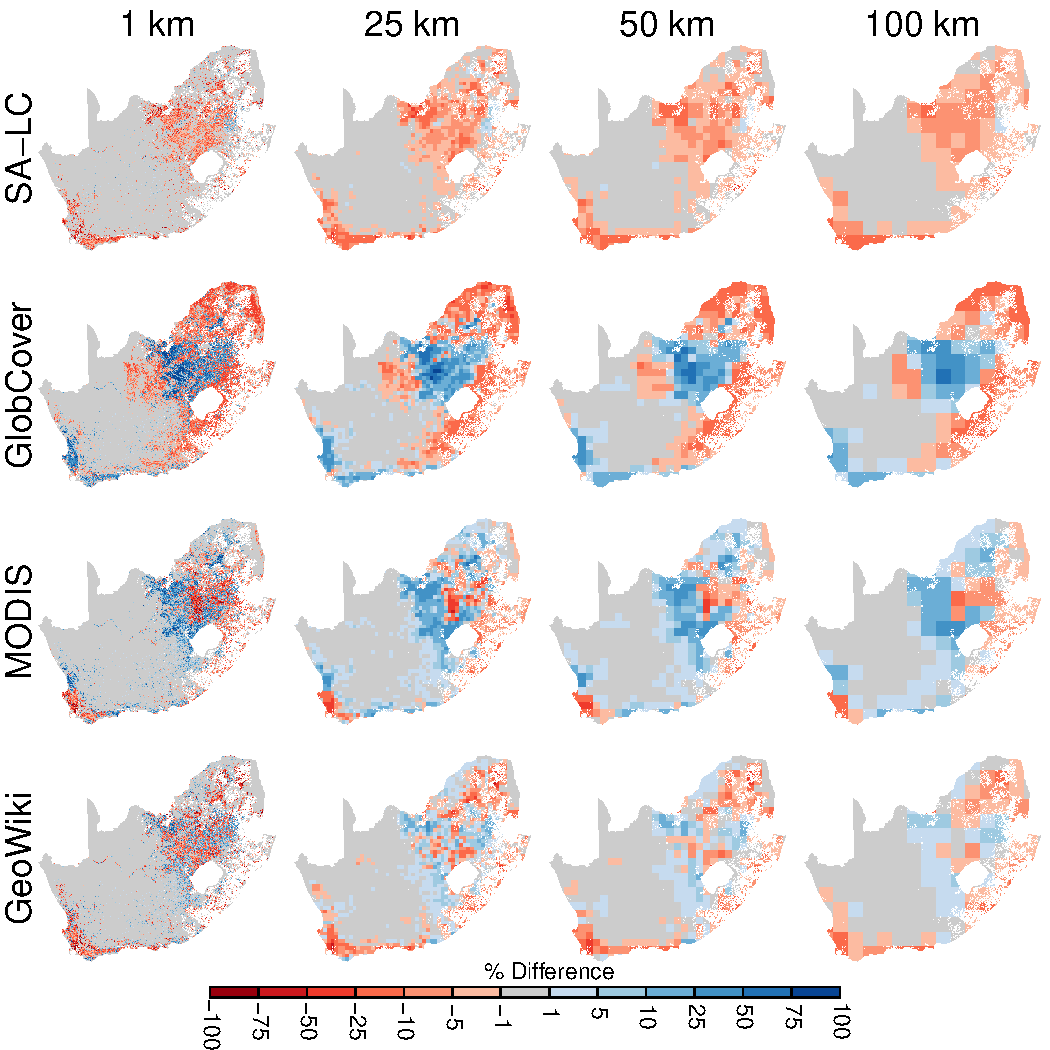
\includegraphics[scale=0.49]{figures/bias_map.pdf}}\quad
%     \subfigure[random caption 1]{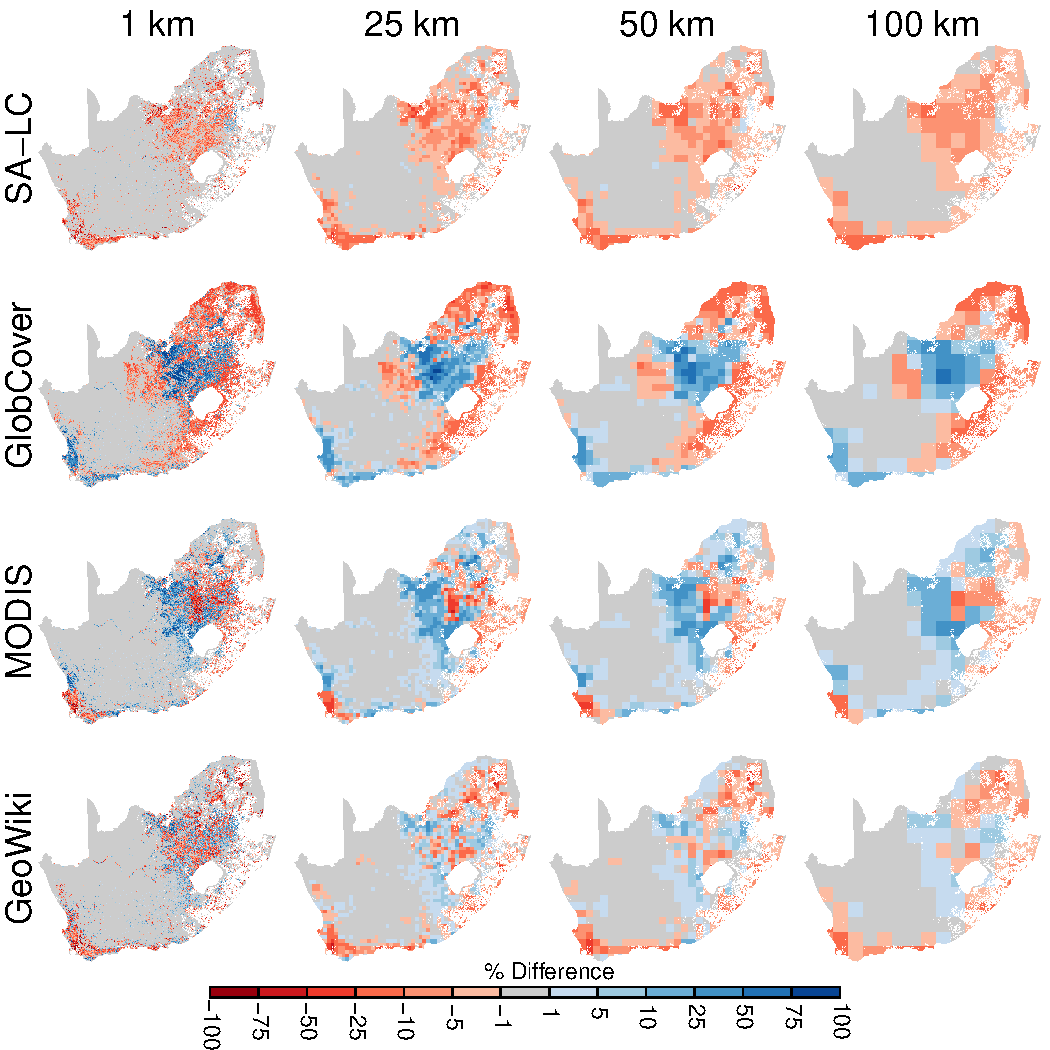
\includegraphics[scale=0.49]{figures/bias_map.pdf}}
%\end{figure*}

\linenumbers
The most pronounced errors were in the MODIS and GlobCover maps, which showed large positive residuals in the center of the country where cropland is most concentrated (blue areas in Fig. 1A), and negative residuals (red areas) along the eastern and northern margins.
These patterns translated into substantial map bias (Fig. 1.B), with GlobCover and MODIS mean error (weighted by the reference cropland density) exceeding 45\% and 25\% respectively at 1 km resolution, meaning that each map tends to underestimate cropland by that amount at that resolution. This bias declined with each level of map aggregation, being reduced to nearly 15\% for GlobCover and 5\% for MODIS at 100 km. The magnitude of (density weighted) mean absolute error (MAE) was somewhat higher in all cases. The GeoWiki map, in contrast, was the least biased overall, showing just a ~7\% bias at 1 km and near 0 for all other scales of aggregation, although its accuracy (23\% MAE) was only half as good as SA-LC's at 1 km (11\% MAE), which despite its uniform overestimation bias (Fig. 1A) was the most accurate map at aggregation scales $<10$km. Above this, GeoWiki became slightly more accurate, having $<$5\% MAE at 100 km resolution. The reason GeoWiki had relatively poor accuracy at 1 km resolution was due to the heterogeneity of residuals, which traded between positive and negative residuals over short distances, thereby inflating MAE at this scale.  

\subsection{Error and landcover density}
Given that landcover characteristics can influence landcover map quality \cite{see_improved_2015, estes_diylandcover:_2015, debats_generalized_????}, we set out to elucidate the relationship between cropland configuration and map error.  We first calculated the average 1 km reference cropland percentage within each of South Africa's 354 magisterial districts (the finest administrative unit, averaging 3,445 km$^2$; SI), which yielded a landscape-scaled metric of characteristic cropland density, and similarly calculated the district-wise MAE for each test map. 

We then used a generalized additive model to evaluate the shape of the relationship between district MAE and cropland density. The model shows that map accuracy is typically lowest at intermediate levels of cropland density (50-60\% cover) for all but the GlobCover map (where accuracy continues to decline with cropland cover), and is highest when the landscape is dominated either by cropland or by another type (Fig. 2). In other words, accuracy is generally lowest when cropland cover is mixed evenly with other cover types. GlobCover's accuracy continued to decrease with cropland density because the dominant agricultural cover class contributing to the test map was defined as 50-70\% crops mingled with other vegetation, thus the maximum percentage was constrained by this mixture range.  

\section{The impact of map error on physical analyses}
\subsection{Estimating vegetative carbon stocks}
To understand the carbon cycle and climate forcing due to land use change, it is important to have accurate, high resolution maps of vegetative carbon stocks \cite[][]{searchinger_high_2015}. One widely used vegetative carbon dataset is that of \cite{ruesch_new_2008}, who mapped estimated carbon density values for different vegetation types to the classes of a global landcover product. The resulting data were intended to provide a baseline for climate policy by the Intergovernmental Panel on Climate Change (IPCC), as well as input to other land use and biogeochemical analyses \cite{ruesch_new_2008}. 

%\vspace{-0.75 cm}
\begin{figure}[!h]
\centerline{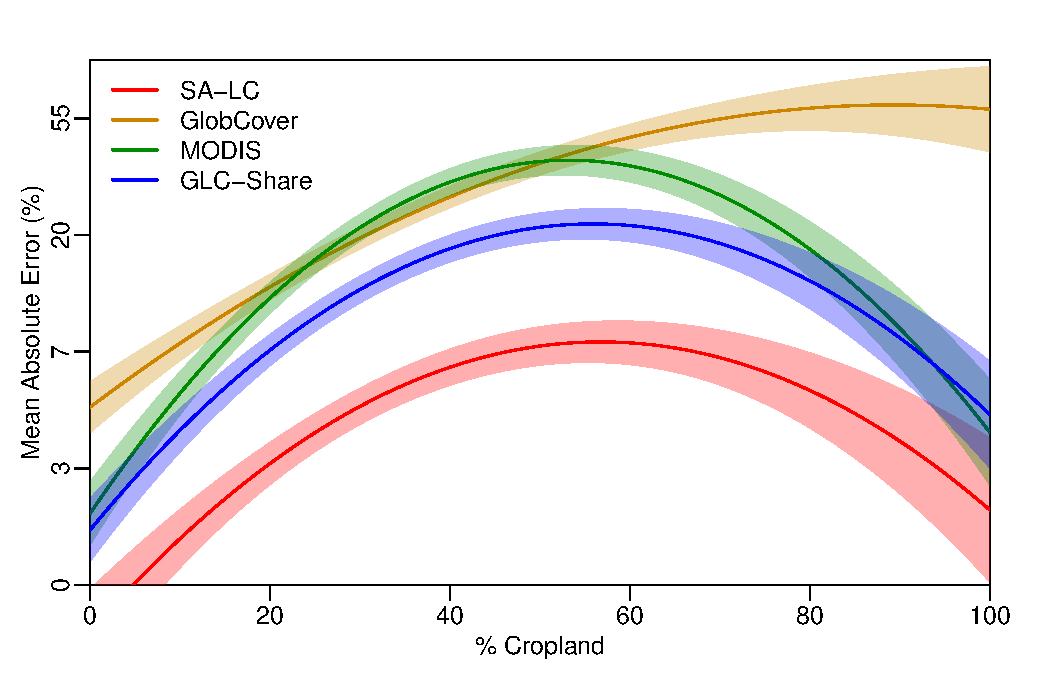
\includegraphics[width=.5\textwidth]{figures/biases_md_lnorm_gam_mu0.pdf}}
\caption{The relationship between map accuracy (the mean absolute error) in test maps and the actual cropland cover within agricultural landscapes (reference map pixels having $>$0.5\% cropland), here defined by the boundaries of magisterial districts (n = 345), as fit with a generalized additive model. Prediction curves are color-coded to the different test maps, with the solid line indicating predicted absolute bias, and the lighter shading the standard error of the coefficients.}\label{afoto2}
\end{figure}

%\vspace{-1 cm}
We followed this method to create vegetative carbon maps for South Africa. Since our maps represented cropland percentage, we developed several variants by assigning the carbon densities of different vegetation types (forest, secondary forest, shrubland, grassland, and sparse vegetation \cite{ruesch_new_2008}) to the non-cropland fraction of our maps. These hypothetical maps represented the range in potential carbon densities, and allowed us to investigate how carbon estimates can vary as a function of i) test map errors and ii) the properties of neighboring cover types. To assess carbon estimation error, we subtracted test map-derived carbon maps from those based on the reference map, and calculated bias and accuracy scores. 

The spatial patterns of test map errors transmitted into carbon estimation errors, but the sign varied as a function of the density of carbon adjacent to croplands (SI). Where cropland was underestimated and the surrounding cover type was more carbon dense than cropland, carbon density was overestimated, but when the cover type was less dense than croplands (e.g. sparse vegetation), then carbon density was underestimated. The inverse was true where cropland was overestimated. 

The magnitude of carbon errors varied as a function of the carbon density of surrounding cover, as demonstrated by the bias statistics (Fig. 3). Bias was near zero when grassland was the adjacent cover type (SI), as its carbon density is nearly the same as cropland. However, when forest was adjacent then bias was a three- to five-fold multiple of cropland map bias (Fig. 1B). At the most extreme, GlobCover's bias was -276\% at 1 km, but even SA-LC and GeoWiki had biases of 22\% and -50\%, respectively. Bias could be substantial even for the least carbon dense vegetation type (sparse), as evidenced by the 15-25\% bias at 1 km for MODIS and GlobCover under this class.  The mean bias across the different potential adjacent vegetation classes ranged between -20 for GeoWiki and -123\% for GlobCover at 1 km (with MODIS in between these), while SA-LC's average bias was 11\%.  Biases declined fairly rapidly with aggregation, with all datasets having an average (across cover types) bias magnitude of less than 10\% by 25 km of aggregation, except for GlobCover, which was -12\% at 100 km (SI).  As with cropland percentages, GeoWiki produced the least biased carbon density estimates above above 1 km resolution. 

In terms of accuracy, MAE values were essentially the same as bias magnitudes, except for GeoWiki's, which were twice as large. The average MAE across vegetation classes was 47\% at 1 km, dropping to $<$10 only with 25 km of aggregation. In contrast, SA-LC's carbon estimates were twice as accurate at 1 km, and was slightly more accurate up to 25 km of aggregation were GeoWiki achieved parity.  

%\vspace{-0.75 cm}
\begin{figure}[!h]
\centerline{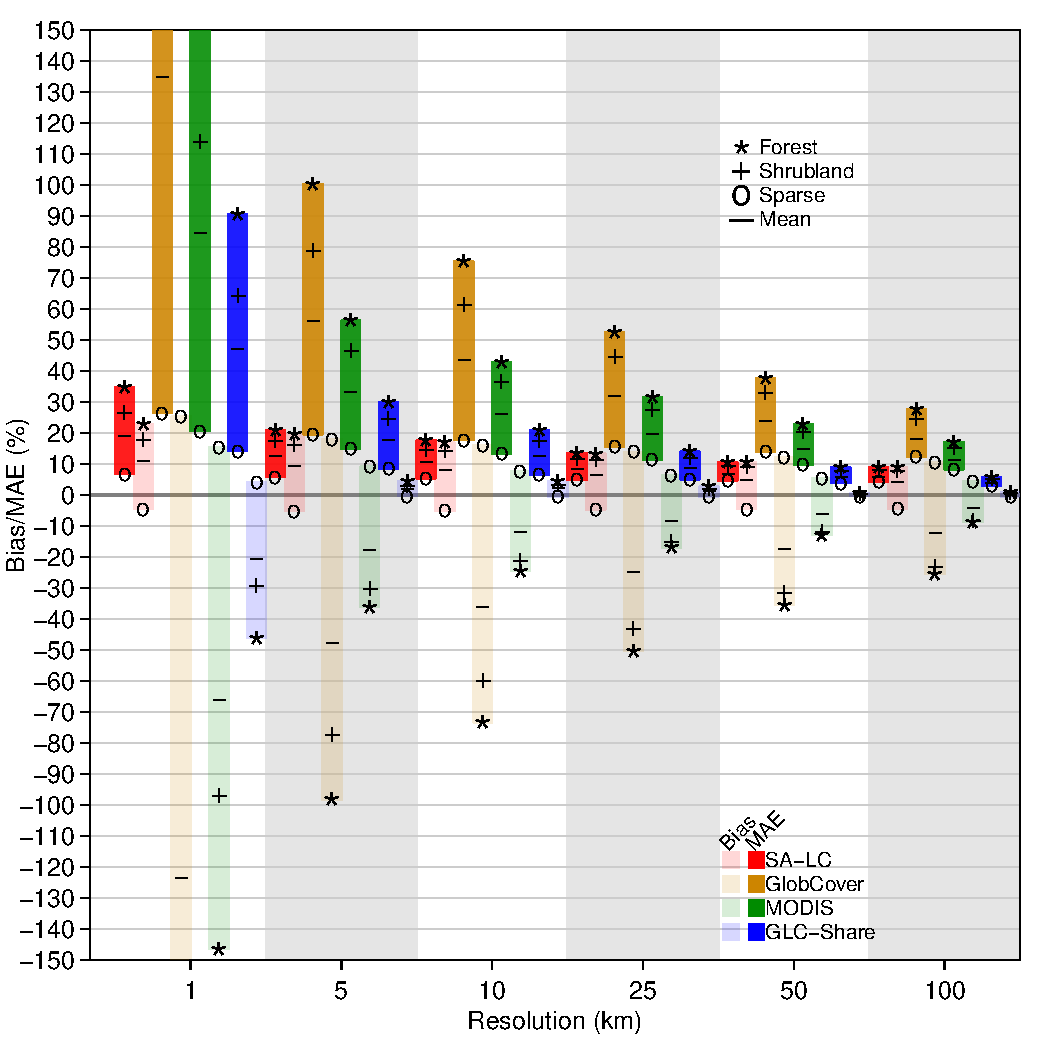
\includegraphics[width=.5\textwidth]{figures/carbon_veg_scalew.pdf}}
\caption{Biases and accuracies (mean absolute errors) of carbon densities derived from cropland maps, calculated as percents relative to the reference map. Bias estimates (represented by symbols) fall within the semi-transparent floating bars, while accuracies are contained in the solid bars. Bar colors are coded to specific cropland map, symbols indicate which cover type was used to calculate cropland-adjacent carbon density. The bar represents the mean biases calculated across each of the 5 cover types. Shrubland and grassland bias values were near zero, while secondary forest values were close to forest values, and thus these are not shown for display clarity (but see Table S2). MODIS and GlobCover values at 1 km exceeding the plot's Y limits are provided near their truncated tops.}
\label{afoto}
\end{figure}

\subsection{Evapotranspiration estimates}
Accurate estimation of hydrological fluxes is critical to understanding how land-atmosphere interactions impact the climate system and runoff \cite{liang_simple_1994}. Land surface hydrological models, such as the Variable Infiltration Capacity \cite{liang_simple_1994}, are used to simulate these processes, and depend on landcover maps to provide information on the characteristics of vegetation and other materials covering the surface, as these govern the rates of runoff, infiltration, and evapo-transpiration. We used the VIC model to generate 25 km estimates of monthly evapotranspiration throughout South Africa, and examined how these were impacted by error in the test maps, which were used to determine landcover-specific values for leaf area index (LAI), plant rooting depth, aerodynamic roughness, and several other variables that VIC uses to partition water vapor fluxes into their evaporative and transpirative components. 

Compared to the carbon analysis, the bias and accuracy in evapotranspiration (ET) calculated using the VIC model was negligible, averaging less than than +/-2\%. However, there were several error hotspots in the resulting ET residual maps (Fig. 4). The most pronounced of these were the 5-15\% overestimates in the center of the country caused when VIC was initialized with MODIS and GlobCover, while overestimates along the southern and western coasts reached 25\%. These locations correspond primarily to the margins of major crop production regions--in the center is the westernmost boundary of the summer rainfall growing region, marked approximately by the 400 mm isohyet, where maize is the primary crop. The west coast hotspot falls at the western edge of the wheat-dominated winter rainfall region \cite{hardy_rainfed_2011}, where growing season rainfall is approximately 200 mm. 

SA-LC and GeoWiki also resulted in ET errors estimates along the southern and western coasts, but here the tendency was to underestimate ET, while biases in the center of the country were either negligible to absent.  All but MODIS underestimated ET by 5-15\% in the northern tip of the country.  


%\begin{figure*}[!b]
%\centering
%  \begin{minipage}[b]{.45\linewidth}
%    \centerline{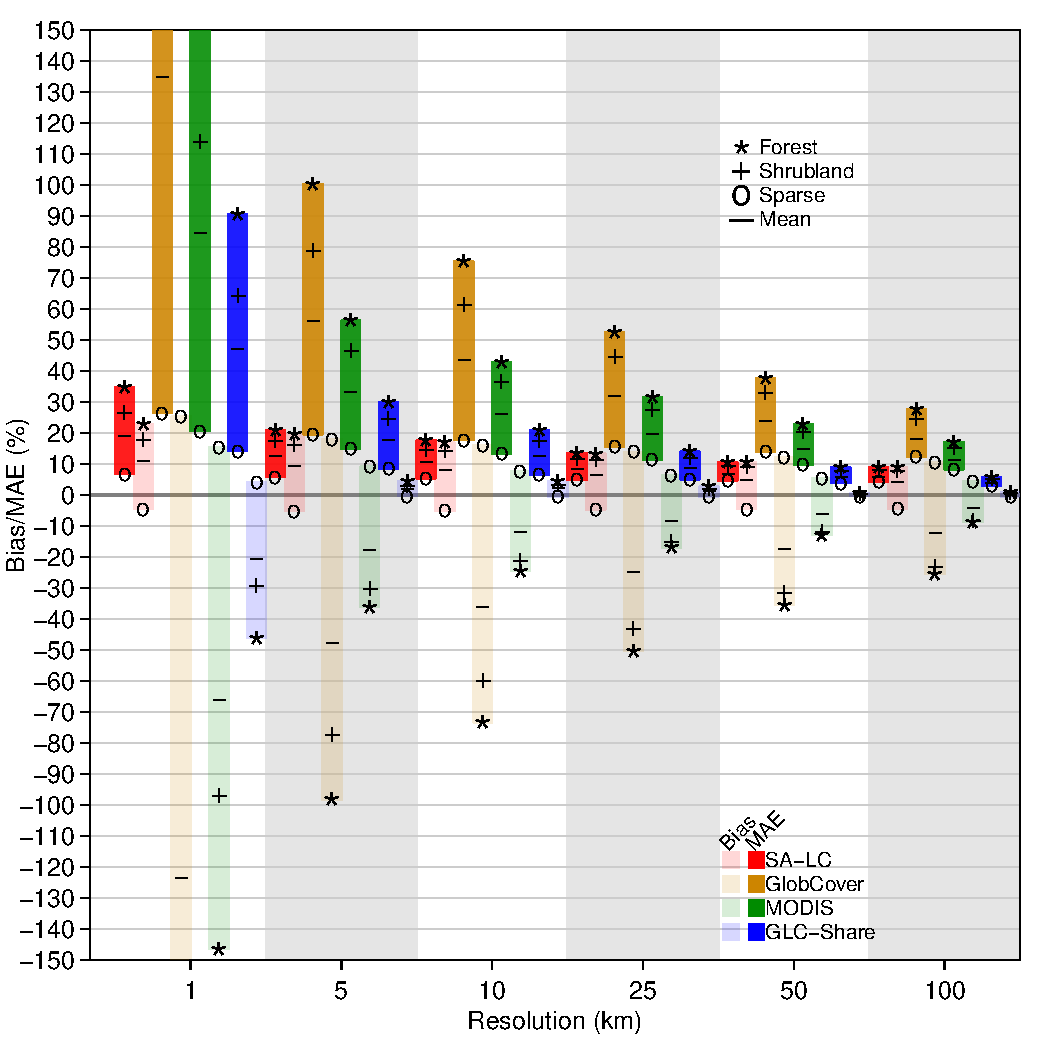
\includegraphics[scale=0.51]{figures/carbon_veg_scalew.pdf}}
%    \caption{Caption}
%    \label{afoto3}
%  \end{minipage}\hfill%\qquad
%  \begin{minipage}[b]{.45\linewidth}
%    \centerline{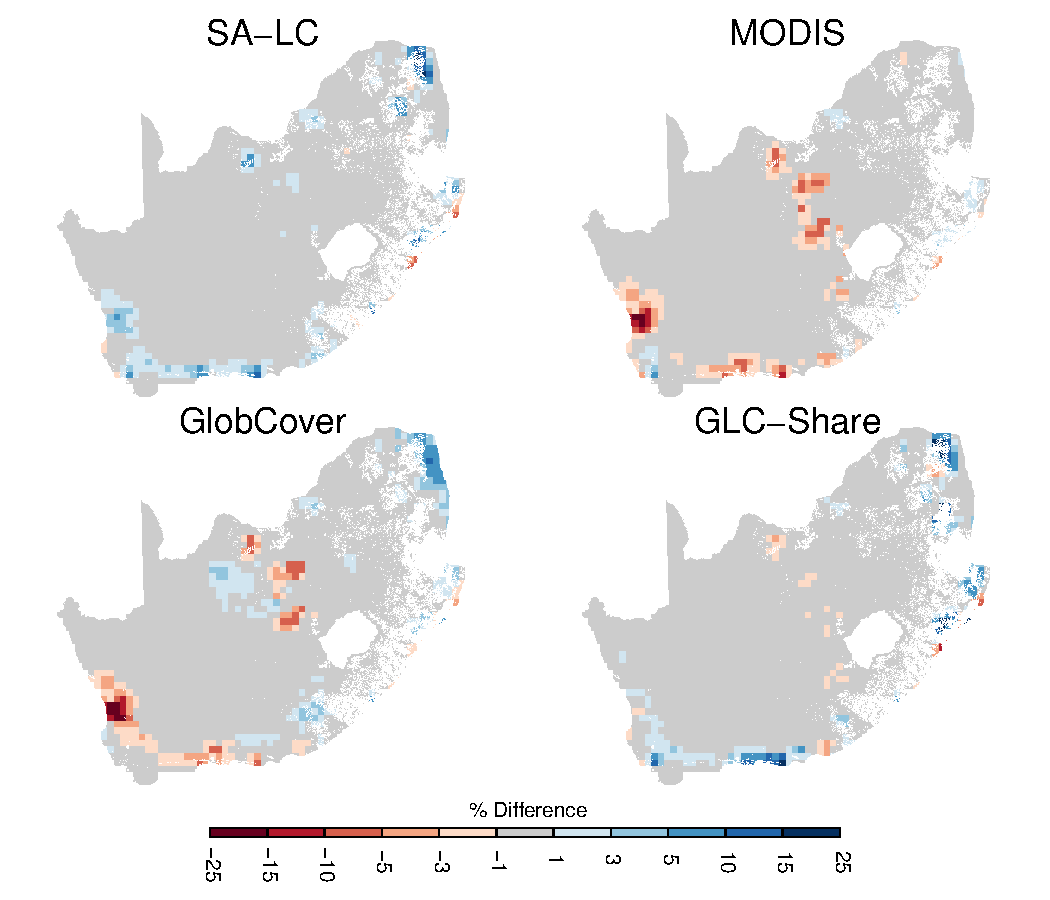
\includegraphics[scale=0.51]{figures/et_bias_map.pdf}}
%    \caption{Caption 2}
%    \label{afoto4}
%  \end{minipage}
%\end{figure*}

%\vspace{-0.75 cm}
\begin{figure}[!h]
\centerline{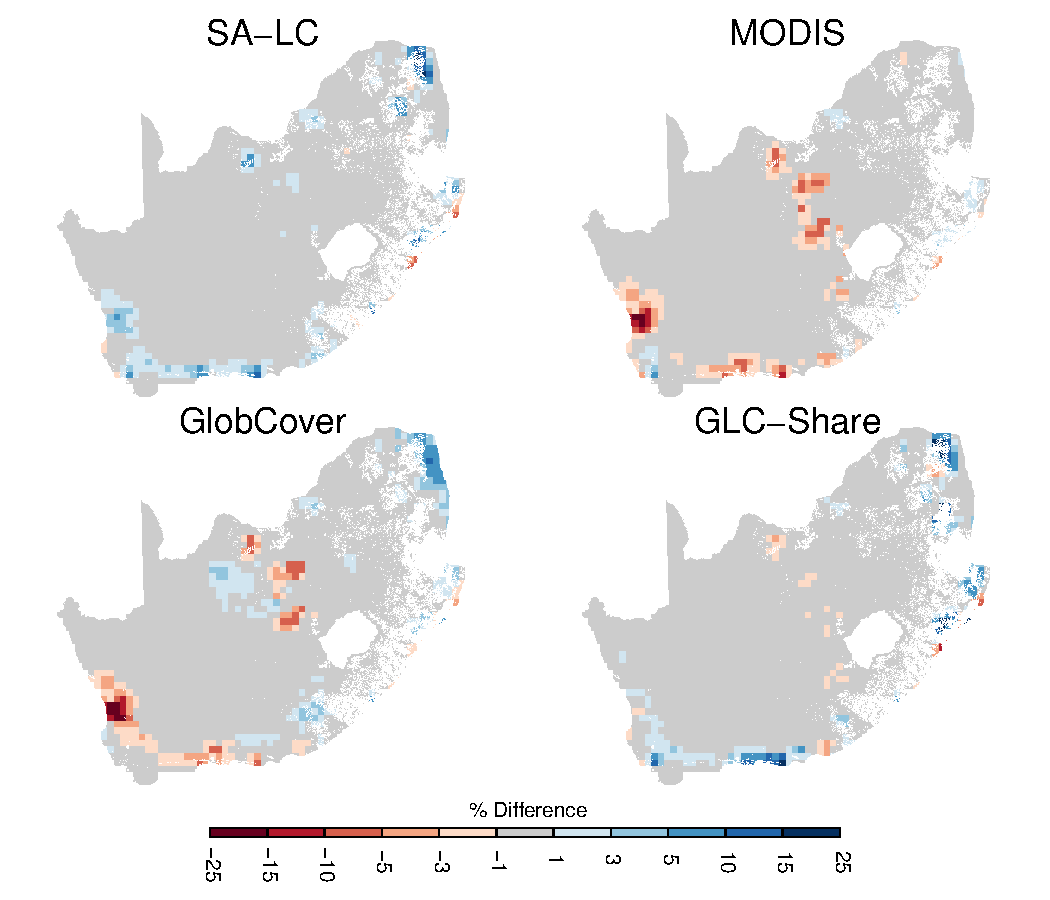
\includegraphics[width=.5\textwidth]{figures/et_bias_map.pdf}}
\caption{Differences in annual mean evapotranspiration estimates from 29-year runs of the VIC land surface hydrology model when initialized with LAI response curves derived from the reference map, versus those from the four test maps.}\label{afoto}
\end{figure}

\section{Socio-economic analyses}
\subsection{Gridded crop yield and production data}
The spatial variability of crop productivity and production is critical for understanding a host of social, economic, and environmental issues, such as food security, trade, and the potential for agricultural expansion and intensification \cite{licker_mind_2010,monfreda_farming_2008}. The most reliable source of such data are national to sub-national agricultural statistics, which are provided for relatively coarse-scaled administrative boundaries. To obtain higher spatial resolutions, efforts have been made to disaggregate these statistics using gridded landcover data \cite{ramankutty_farming_2008,monfreda_farming_2008}. These disaggregated datasets, which are constrained to match the agricultural statistics within the boundaries of the areas for which they are reported, have seen increasing use because they are considered to be more accurate than single source methods, and provide consistent data on which to base studies of global change \cite{ramankutty_farming_2008, see_improved_2015}

We used these same methods  \cite{ramankutty_farming_2008,monfreda_farming_2008} to disaggregate maize harvested area (South Africa's largest crop \cite{estes_projected_2013}) on top of our reference and cropland maps, followed by yields, which were assigned to cells have harvested areas greater than zero. We then used these two layers to calculate maize production, and further aggregated the yield and production grids to 5, 10, 25, 50, and 100 km resolutions before quantifying the bias and accuracy of each test map's yield and production values. In this case, we could not convert cell-wise errors into percentages of the reference map values (because many cells had zero values for one map but not the other), so calculated bias and accuracy from the map residuals and then normalized their values to the reference map means. 

Maize yields disaggregated onto the test maps showed some marked differences relative to the reference map, but only at the margins of the major crop production areas where cropland is sparser (SI). These differences resulted when a yield value was mapped onto a grid cell where the reference map had no harvested area, and thus zero yield. In more densely cropped areas, such discrepancies were less frequent because both the reference and test maps were both likely to have some maize harvested area, and therefore a yield value.  Yield biases were thus fairly low (and accuracy high), with the largest being 20\% for MODIS at 1 km, following by GlobCover with 10\% (Fig. 5). These dropped to below 10\% with aggregation.  

Production biases were generally slightly higher, but still low, for most datasets, with the exception of GlobCover, which had an gigantic underestimation bias of $>$60\% (relative to mean production) at 1 km, which remained above 10\% even at 100 km of aggregation. MODIS production bias was above 20\% at 1 km, but declined to below 10\% at higher levels of aggregation.  

The accuracy of production estimates was another story. Here all datasets but SA-LC had MAE values of 30\% or higher below 25 km of aggregation (Fig. 5), reaching as high at 100, 65, and 45\% at 1 km for GlobCover, MODIS, and GeoWiki, respectively. Only GeoWiki's MAE fell below 10\% with 100 km of aggregation.  SA-LC estimated production was most accurate, having between 10-20\% MAE between 1 and 10 km, and $<$10\% at 25 km and higher.  This low accuracy relative to the gridded yield measures relates to the disaggregation process for harvested area, which allocates a fractional value to each pixel, which is itself a fraction.  The process of adjusting the gridded values so that their total match the statistics from which they are derived does not adjust map errors relative to the reference map, and the constraint in fact appears to shorten the distance between negative and positive residuals (SI), thereby increasing absolute errors.  

\subsection{Agent-based simulation of food security}
Spatially-explicit agent-based model (ABMs) are frequently employed to understand land use decision-making and socio-ecological systems, often to facilitate improved policy, particularly in the arena of human development \cite{berger_creating_2006}. To obtain valid insight into the functioning of such systems, it is important to calibrate an ABM to empirical data describing the characteristics of land and land users, so that the model realistic represents the social and biophysical features of the study region \cite{berger_creating_2006}. In our example, we used an ABM of household food security that simulates the food production by individual farming households (the agents) in response to weather and management capacity, which varies as a function of household resources, including the area and physical characteristics of fields \cite{chen_dependency_2013}. The model is initialized such that each household is allocated its designated share of cropland, and then produces a crop over the course of one to many seasons. Like many spatial ABMs, the model is computationally intensive, and thus run over smaller geographic domains (e.g. districts, rather than an entire country) and at higher spatial resolutions (10s to 100s of meters) in order to represent the different land units of single farmers. To match these computational characteristics, we selected four contiguous magisterial districts (ranging from 1,040-1,343 km$^2$, Fig. S8) in the eastern part of the country with 28-45\% of their areas devoted to cropland. The initialization process iteratively assigns households to the landscape using a function that factors in neighbor and cropland proximity, to ensure that households are grouped into communities and that their fields are within a realistic proximity. The number of households and the cropland area per household is derived from survey data of communities where all cropland is owned. The model is thus considered to well calibrated when all households are allocated their appropriate area of cropland, and all cropland is occupied. 

%\vspace{-0.5 cm}
\begin{figure}[!hb]
%\vspace{-0.75 cm}
\centerline{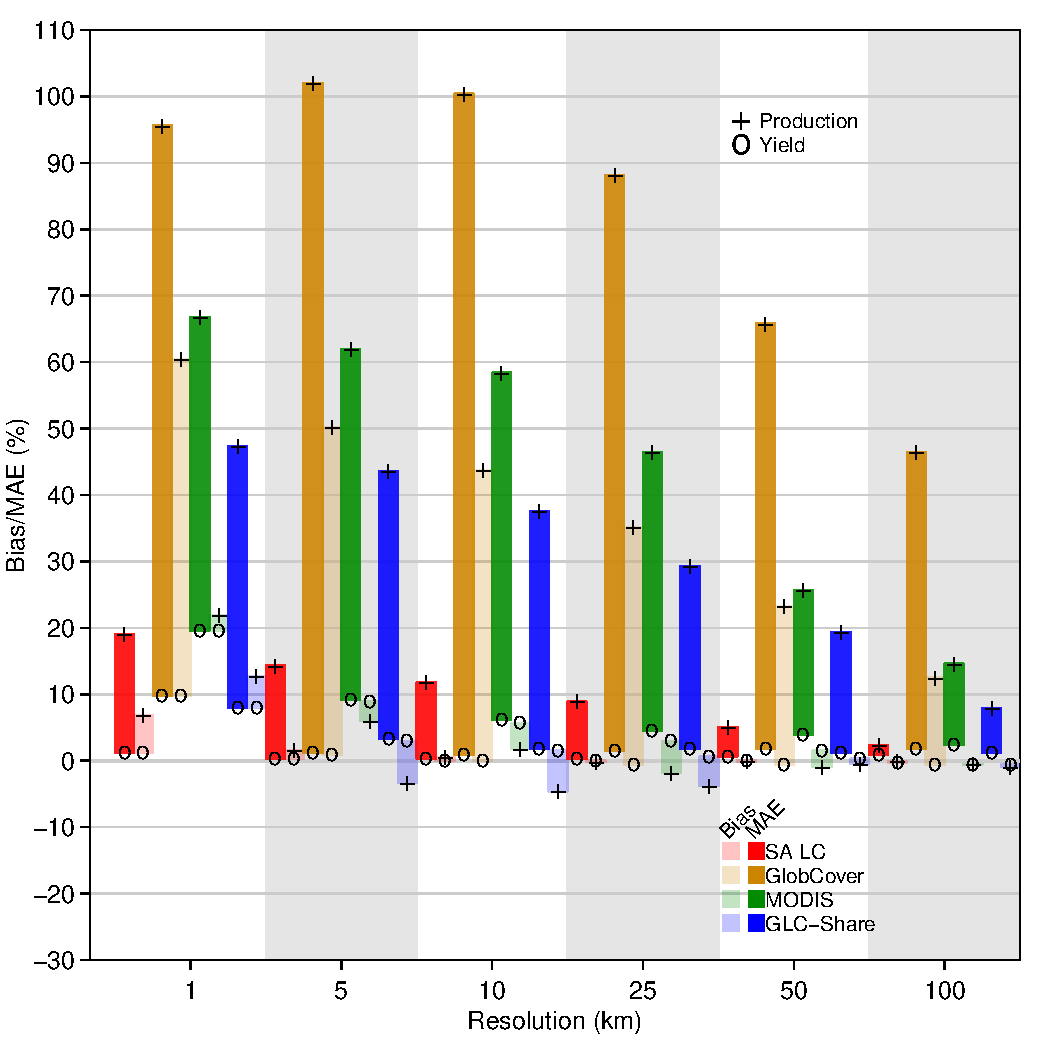
\includegraphics[width=0.5\textwidth]{figures/yield_prod_bias.pdf}}
\caption{Bias (mean error) and accuracy (mean absolute error [MAE]) in disaggregated maize yield and production estimates. Bias estimates (represented by symbols) fall within the semi-transparent bars, mean absolute errors in the solid bars, with bar colors coded to specific cropland maps.  Symbols code the different variables (production and yield), normalized to their respective means.}
\label{afoto}
\end{figure}

We used the reference map and each cropland map to separately initialize the model, and examined how map errors impacted the land allocation process and household food production estimates. We examined three variables: the percent of unallocated cropland, land deficit, and food deficit. The percent of unallocated cropland measures how effective the model was in matching household agents to available cropland resources. Where error was negative (indicating a cropland overestimate by the test maps), the amount of land left unallocated had a straight one-to-one relationship with the percentage of overestimation (Fig. 6A). When cropland was underestimated, no land was left unallocated until the underestimation exceeded 50\%. The MODIS-based simulation for districts 1 and 2 was most pronounced for this tendency, where 5-10\% of cropland remaining unallocated despite the fact that cropland with such a high cropland underestimate (85\%) the majority of households were not allocated cropland. This curious relationship occurred because croplands tend to cluster, and when underestimated clusters tend to be small, resulting in islands of cropland that fall outside of the search radius within which cropland is sought when agents are seeded onto the landscape. 

The second measure, land deficit, describes the amount of land that the model should have assigned but couldn't due to the mismatch between the cropland map and the statistical estimate of cropland holdings. Land deficit increased exponentially in relation to cropland underestimation--reaching around 800\% for MODIS in districts 1 and 2 (Fig. 6B)--and would become infinite in the case of a 100\% underestimate. This contrasted with the third measure, food deficit, the shortfall in the average amount of food that should have been produced by each household but wasn't because of the land deficit; this particular deficit increased linearly with the percentage of cropland underestimate (Fig. 6C). 

%randomly siting 100 household agents within each district, and allocating the nearest two cropland pixels to each household. The remaining agents are then iteratively assigned unallocated cropland pixels within a 1.5 km radius of existing agents' fields, and this process continues until all agents are assigned cropland, or all available cropland is allocated. This initialization process 
%\FloatBarrier

\begin{figure}[!ht]
\centerline{\includegraphics[width=.5\textwidth]{figures/figure6.pdf}}
\caption{Biases in agent-based model results relative to the district-wise errors (as a percent) in total cropland area, in terms of A) the percent of cropland in each district that was not allocated to any household, B) the land deficit, or the percent of cropland that should have been allocated to households but wasn't, and C) the food deficit, or the average food production across households resulting from inadequate cropland allocation. Dot sizes correspond to district numbers, colors represent the landcover map.}
\label{afoto}
\end{figure}

\section{Discussion}
This spatially comprehensive, bottom-up assessment of landcover map bias and accuracy provides new insight into their extent, causes, and consequences for understanding global change, made possible by a unique, high accuracy dataset that likely provides the truest measure of cropland area and distribution currently available for this region. This dataset is not perfect, being affected by the map-makers' occasional interpretation errors (mostly of omission), while some of the error we identified may be due to slight temporal mismatches between the reference and test datasets. However, our assessment (SI) suggests that these errors are small, and do not appreciably impact our findings, which is bolstered by previous work showing the substantial errors and inconsistencies between landcover maps \cite{fritz_comparison_2010,gross_monitoring_2013}. These previous studies, which were conducted over broader extents than ours, also indicate that our findings should be generalizable beyond South Africa's borders, particularly to more rapidly developing, data poor regions.

\subsection{General guidelines for selecting and using landcover data}
Our results suggest several guidelines for selecting and using landcover data in global change research. First, landcover products derived from coarse resolution sensors, such as MODIS and GlobCover, need substantial aggregation to reduce the large biases and inaccuracies that manifest at finer resolutions. Researchers might need to use these datasets for a variety of reasons, for instance, because they provide consistent, multiple landcover classes at a global scale, or allow changes to be tracked across large scales over time \cite{luoto_predicting_2004}. The appropriate scale of aggregation then depends on which error property the user wants to minimize. For instance, if the objective is to minimize systematic errors in order to calculate an unbiased mean (e.g. average carbon density), then at least 50-100 km of aggregation is needed to reduce map bias to within +/-10\% (Fig. 1B, 3). If the user wants to maximize accuracy (accuracy is important for comparing differences between locations on a single map, or between dates at fixed locations), then even coarser aggregations are needed to reduce mean absolute error below 10\% (Fig. 1, 3, 5).  

The characteristics of cover at the landscape scale may also require greater levels of aggregation to achieve sufficient accuracy. We found that accuracy is lowest where mixing of cover types is greatest (Fig. 2), a result echoed in an Africa-wide change detection study made with MODIS \cite{gross_monitoring_2013}. Outside of South Africa, where smallholder-driven agriculture predominates \cite{lambin_estimating_????} such mixed landscapes are more common, thus greater levels of aggregation may be needed over these areas. Coarser aggregations are also necessary if the cover type of interest belongs primarily to a mixed class (as with GlobCover). This leads to underestimation bias (Fig. 2) and high inaccuracy, which will persist until the aggregated pixel exceeds the characteristic size of the geographical area within which the cover type dominates. In South Africa's farming regions, this can exceed 1000 km$^2$. 

Maps derived from higher resolution sensors, such as the SA-LC dataset, do not have this mixture problem because the pixels are fine enough to be assigned to a single cover type. This characteristic leads to higher accuracy, which is what we observed here: the SA-LC dataset needed the least aggregation--just 5-10 km--to achieve $<$10\% MAE in most of the example applications we tested (note, however, another guideline in this result: even with high resolution maps some aggregation is needed to achieve higher accuracy).

%needed This observation leads to a second rule of thumb: users should select datasets from higher resolution sensors where possible (assuming they were carefully developed), as these needed much less aggregation to return accurate estimates for most applications we tested here. For $<$10\% MAE, just 5-10 km of aggregation were needed (however, this is still much coarser than the 30 m resolution of the sensor itself).    

Unfortunately, Landsat-scaled maps are typically developed for specific countries, using varying methods, and can be hard to obtain (an exception to this is the newly released GLC30, which has a reported classification accuracy of 80\% \cite{chen_global_2015}). Our results also suggest that, despite their higher accuracy, they are not necessarily the least biased maps. Except for a few results (notably the 1 km carbon and maize production estimates), GeoWiki-based maps had the least amount of bias across most scales. GeoWiki's lower bias results from its process of calibrating the cropland percentages to reported agricultural statistics \cite{fritz_cropland_2011,fritz_mapping_2015}.  The procedure is similar to the one we used in disaggregating maize harvested areas \cite{ramankutty_farming_2008, monfreda_farming_2008}, which led to fairly unbiased estimates of maize production and yield (Fig. 5) above 1 km (except for GlobCover's production estimates). This result, together with GeoWiki's unbiased cropland estimates (Fig 1.B), indicates the value of fusing inventory data with remote sensing to reduce map bias. 

%The consensus method mirrors the ensemble averaging used by other fields (e.g. crop \cite{asseng_uncertainty_2013}, climate \cite{giorgi_calculation_2002}, and ecological modeling \cite{araujo_ensemble_2007}) to increase prediction confidence.

Of course, for the constraint to be effective, the inventory data themselves must be faithful to reality, but in many places, particularly Africa, agricultural statistics are suspect \cite{carletto_emperor_2013, fao_action_2013}, which is a vulnerability of the fusion approach \cite{see_improved_2015}. Beyond this limitation, this method does not improve map accuracy, which is evident in GeoWiki's relatively high MAE for cropland percentage at 1 km (23\%, Fig. 1B), and by all maps' (except SA-LC's) highly inaccurate maize production estimates (Fig. 5). The reason that accuracy is not improved is because the statistical constraint cannot correct the omission and commission errors within the landcover maps.  

These last observations suggest two further guidelines: 1) for high accuracy, users should select well-validated datasets from higher resolution sensors--this option should be increasingly available as computational power grows and high resolution image archives expand \cite{hansen_high-resolution_2013,chen_global_2015}; 2) where low bias is needed over large areas, the best option is to use newer generation, statistically constrained maps such as GeoWiki (and possibly the GLC-Share \footnote{GLC-Share. www.glcn.org} datasets for other cover types). But in either case some aggregation--5-25 km, depending on application and whether low bias or high accuracy is the objective--will still likely be necessary to achieve sufficiently low error. Additionally, these higher accuracy, lower bias product are made infrequently, thus applications requiring high frequency landcover data will depend on MODIS and confreres, as previously mentioned, and therefore much coarser aggregations.  

%GeoWiki was the most accurate among the large scale landcover products, but its improvement is related to the map consensus methods, which can correct for omission or commission errors made by the classifier. 

\subsection{Implications for global change analyses}
Besides the preceding landcover data selection and usage guidelines, our findings also have broader implications for global change analyses and associated policy decisions. The simpler, most direct uses of landcover data have substantial to skew our understanding of global change processes. For example, the global carbon carbon density map of \cite{ruesch_new_2008}, of which we created facsimiles here, has been widely used, but our results suggest that any analyses of the spatial variability of carbon stocks, or of mean carbon densities, can be highly misleading if the map is not first sufficiently aggregated. For example, a study of deforestation risks in the Democratic Republic of the Congo estimated forest rents as a function of carbon densities based on this map. Although the map was aggregated to $\sim$50 km, we found that mean absolute errors can still reach 40\% at this scale (Fig. 3). The same carbon map provided country-specific mean forest carbon densities for an evaluation of climate mitigation policies \cite{cattaneo_international_2010}, which our results suggest could be underestimated by 70\% (Fig. 3). In contrast to these, an assessment of the congruence between carbon and biodiversity \cite{strassburg_global_2010} aggregated the carbon data to $\sim$110 km resolution, where accuracy is much higher. 

A related example can be seen in studies that create high resolution maps (10 km) showing the potential food production benefit of closing yield gaps \cite[e.g. Figure 3 in][]{foley_solutions_2011}. Such maps give an inflated sense of the precision with which such locations can be identified. Although the study in this example is careful to report aggregated statistics, in which we can have greater confidence, it is not inconceivable that the maps themselves are used to inform policy. For this reason, it is advisable to degrade maps until their accuracy is of an acceptable standard (i.e. $\geq$100 km). 

Aggregating until acceptable accuracy is achieved will be particularly important in growing efforts to find tradeoffs between agricultural development and ecological protection \cite[e.g.][]{searchinger_high_2015,west_trading_2010}. Finding win-wins fundamentally requires accurate, fine-scale data in order to identify ``win-win'' solutions, which are comprised of areas where there is some deviation from an expected relationship; for example, an area of unusually low carbon density but high crop fertility \cite{searchinger_high_2015}. Without sufficient aggregation, it is difficult to know whether such efficiencies are due to real biophysical properties, or simply landcover error. 

What then, of the impacts of landcover data on more complex analysis?  Here the results appear to be mixed. Map error appears to have had little impact on the overall bias and accuracy of VIC's evapotranspiration (ET) estimates, which contrasts with a related study that examined how landcover maps impact rainfall simulations \cite{ge_impacts_2007}. There are two reasons for this. First, map accuracy increased nearly two-fold by aggregating to 25 km, the resolution of VIC. Second, VIC's landcover-derived variables (e.g. LAI curves, effective rooting depth) could dampen the effect of map errors on ET calculations when the values of these variables in the adjacent landcovers are similar to that of cropland, which is the case in much of VIC's landcover scheme for South Africa. In other regions, where the matrix landcover's LAI values depart substantially from cropland's (e.g. in forest), the ET errors would likely be much larger. The carbon example illustrates how cover properties can mute or amplify map error.  

Despite the low values of the overall error metrics, the hotspots of ET errors (Fig. 4) are important, because they occurred at the climatic margins of the major crop growing regions, where a substantial share of farms use irrigation. Since VIC does not simulate irrigation, the magnitude of these errors is likely to have been underestimated, because irrigation substantially increases latent heat flux \cite{sacks_effects_2008}. This also suggests the potential for map error to magnify in a coupled land-atmosphere model (which could explain the difference between this result and that of Ge et al. \cite{ge_impacts_2007}.), and thereby give misleading insight into the climatic effects of land use.     

Relative to the ET example, map errors had a much larger impact on the agent-based model's results. For the model's most important metric of food security--household-level crop production--the result was fairly straightforward for a class of models where the interactions of multiple agents often produce analytically intractable outcomes \cite{janssen_empirically_2006}. In this case, the model was only sensitive to cropland underestimates, which had the perfectly predictable effect of lowering average household food production, which would in turn overstate the degree of food \emph{in}security. Overestimates did not matter in this case, because the number of households remained fixed, and their cropland holdings were constrained to match the survey statistics (but this would matter for models that allow these parameters to vary). Less predictable was the finding that the spatial distribution of cover can impact model parameterization, with land being left unallocated even when needed, thus such models also require spatial, not just statistical, accuracy in their base landcover maps.  

The errors in the cropland data we tested were large, and it is unlikely that current ABM-based studies, mostly of small regions, are based on such inaccurate landcover data. However, as computing power increases, so, too, does the feasible application extent of ABMs, which then become more reliant on larger-scaled, more erroneous, landcover data, with the attendant risk that insights into socio-ecological systems arising from these models could be highly misleading.  

Beyond these examples, there are other applications where landcover map errors could alter understanding and policy. One of these lies in assessments of land availability for agricultural expansion, which could be particularly erroneous if they use a ``residual approach'' \cite{lambin_estimating_????}, where existing cropland and other occupied cover types are used to filter a map of potential suitability. Our results suggest that the pronounced underestimation biases (Fig. 1) we found could inflate land availability estimates, and therefore increase the risk of unjust land allocation policies \cite{rulli_global_2013}. Another example is the growing efforts to minimize the environmental and climate impacts on new agricultural expansion frontiers, particularly Africa's savannas, which requires identifying areas that provide the highest agricultural benefit for the lowest environmental cost \cite{searchinger_high_2015}.  In order to be effective, such analyses must be undertaken at the fine scales--hectares, rather than square kilometers--at which land use decisions are made, thus their value for informing land use policy is contingent on the accuracy of their underlying landcover/land use data \cite{searchinger_high_2015}.

\subsection{The way forward}
Our analysis demonstrates that the landcover data that increasingly inform much global change research and policy can be substantially misleading, depending on the dataset selected, its application case, the scale to which it is aggregated, and whether the insight being drawn from the map depends on how accuracy or low bias. We provide some basic guidelines for selecting and using landcover data that can help increase confidence in the conclusions drawn from landcover-based studies. 

Beyond these guidelines, we recommend updating several important, global-scale datasets using the latest generation landcover maps. For example, rebuilding the widely used cropland distribution and yield maps \cite{monfreda_farming_2008, ramankutty_farming_2008} using the GeoWiki map could substantially improve our knowledge about current global agricultural distribution and productivity. Similarly, reconstructing the carbon map of \cite{ruesch_new_2008} using the GLC-Share datasets (in which GeoWiki provides the cropland layer) would improve our confidence in regional to global assessments of vegetative carbon stocks. Alternatively, the new high-resolution, Landsat-based GLC30 \cite{chen_global_2015}, aggregated and converted to fractional cover classes at 1 km--and fused with high quality national landcover maps, where available \cite[similar to][]{fritz_mapping_2015,fritz_cropland_2011}--may provide a preferable base map for rebuilding these datasets. 

Even more promising are newer approaches that fuse human judgement with expanding high resolution satellite data archives, improved classification algorithms, and expanding computing power. The GeoWiki project and the new high resolution global forest change map \cite{hansen_high-resolution_2013} provide the most prominent examples of these latest methods. Another approach is that of the Mapping Africa project\footnote{http://mappingafrica.princeton.edu}, which, inspired by quality of the reference map used in this study, enlists internet-based workers to manually digitize cropland boundaries \cite{estes_diylandcover:_2015}.  Merging this approach with newer computer vision-based mapping algorithms \cite{debats_generalized_????} is a near-term goal of this project, which will combine the superior capacity of humans to delineate discrete cover types in noisy images \cite{estes_diylandcover:_2015} with the algorithm's speed and ability to classify highly dimensioned image features. These ongoing projects represent the next generation of landcover maps, and offer to greatly improve our understanding of global change. 




% $\theta$ changes from 0 to 1. (see Figure \ref{afoto}).That means we are considering $\theta$  of the form
%For these solutions we have the following

%\begin{remark}
%Note that equation \eqref{theta} specifies  the function $\varphi$
%up to an error of order $\delta$. Theorem 1 provides an evolution
%equation for the function $\varphi$ up to an error of order
%$\delta |log \delta|$.
%\end{remark}

%(see \eqref{weaksol}). 


\begin{materials}
\section{Methods} 
Perhaps it is right {\it SI Materials and Methods}.

Describe weighted mean bias reasons. 

We disaggregated the cropland percentages in all maps to binary cropland/non-cropland cover types with 100 m resolution, which matches the typical field size (1 ha) for smallholder farmers in household survey data (collected in Zambia) used in developing the agent-based model \cite{chen_dependency_2013}. The surveys provided the mean cropland area per household (2.2 ha) and frequencies distribution of cropland area holdings across households (e.g. how many households have 1 ha, 2 ha, etc.). We used these statistics to calculate the ``true'' number of households per district by dividing reference cropland areas by the mean cropland area, and preserved the cropland area distributions by multiplying the total number of households by the frequencies. We then initialized the model, which takes a weighted (by cropland area frequency) random draw of 100 households and places these within the district, assigning each household its required number of ``fields'' (cropland pixels), which must be within 1.5 km of the household's location and not already assigned to another household. This process is iterated until all households are assigned cropland, or all available cropland is allocated. 


The South African government commissioned a whole-country cropland boundary map to enhance its annual collection of agricultural statistics \cite{fourie_better_2009}. The map was made by trained workers who visually interpreted high resolution satellite imagery ($<$5 m SPOT imagery) and manually digitized field boundaries following a standardized mapping protocol. The resulting vectorized field maps, provide a unique, high quality reference dataset describing South African crop field distributions and size classes for the period 2009-2011, and are 97\% accurate in distinguishing cropland from non-cropland at 200 m resolution. We intersected the field vectors with a 1 km grid, and calculated the percent of each cell occupied by fields to create a gridded cropland reference map. 

We extracted the cropland classes from the first three datasets and converted these to 1 km resolution percent cropland estimates, resulting in 4 maps (hereafter simply the ``cropland maps'') to compare to our reference map.  

The first of these was the widely used International Panel on Climate Change's Tier-1 approach for mapping vegetative carbon stocks, as developed by \cite{ruesch_new_2008}. The second was maize yield maps derived by disaggregating district-scale agricultural census data for both maize yield and harvested area \cite[following][]{monfreda_farming_2008,ramankutty_farming_2008}, from which we calculated the third map, gridded maize production estimates. Maps based on these analyses underpin many assessments of crop productivity and production \cite[e.g.][]{foley_solutions_2011,licker_mind_2010}.  

For the first of these, we used the Variable Infiltration Capacity \cite{liang_simple_1994} land surface hydrology model to calculate monthly evapotranspiration, using the reference and cropland maps to adjust landcover-specific leaf area index (LAI) values that VIC uses to partition water vapor fluxes into their evaporative and transpirative components. In the second example, we examined how these map errors impact the land allocation process of an agent-based food security model \cite{chen_dependency_2013}. 

The reference dataset covered all of South Africa's field crop estate, from which we filtered out areas of communally owned farmlands and permanent tree crops to have a common basis of comparison across all landcover products, leaving us with map, after conversion to cropland percentage, that covered or 90\% of South Africa (1,081,000 km$^2$), of which 104,304 km$^2$ 2011 reference map showed a cropland area of 104,304 km$^2$, which the SA-LC and GeoWiki maps overestimated by 31 and 10\%, respectively, and GlobCover and MODIS underestimated by 18 and 23\%.  

from agricultural pixels ($>$0.05\% cropland)

The difference between total carbon stocks for the country made using any of the cropland maps were within +/-3\% of those based on the reference map, regardless of which cover type was adjacent to cropland (Table S1), as the large uncropped area of South Africa (Fig. 1) dilutes the errors within the 

The disaggregated yield and harvested area maps of \cite{monfreda_farming_2008} are built upon cropland fraction maps where the total area is adjusted to match survey-derived cropland area statistics reported for administrative districts \cite[provinces, in South Africa's case][]{ramankutty_farming_2008}. To be consistent with this methodology, we first adjusted our cropland maps according to this procedure, using the reference map to calculate total cropland area for each of South Africa's nine provinces, then updating the pixel-wise cropland percentages in the four cropland maps so that the province-wise sums matched the reference areas \cite[][and see SI]{ramankutty_farming_2008}. Despite this statistical constraint, the updated cropland maps still had substantial errors that were similar in pattern (Fig. S5) to those in the unadjusted maps (Fig. 1), and we evaluated how these residuals affected gridded estimates of the yield and production of maize, South Africa's largest crop \cite{estes_comparing_2013}. To create these maps, we followed \cite{monfreda_farming_2008} by disaggregating district-level (n = 354, mean area = 3,445 km$^2$) agricultural census data \cite{statistics_south_africa_commercial_2007} for maize (South Africa's largest crop by area, \cite{estes_comparing_2013}) yield and harvested area, aggregated each set of maps, and multiplied the two to calculate production at each scale. 

(which is constrained by an absolute distance and the proximity of other agents) 

\section{Digital RCD Analysis} 
\end{materials}

\appendix[App 1]

\appendix
This is an example of an appendix without a title.

\begin{acknowledgments}
I thank everyone tearfully. 
\end{acknowledgments}


% bib solution from here
% http://tex.stackexchange.com/questions/167650/is-there-a-more-recent-bibliography-style-file-bst-for-pnas
% https://github.com/jburon/pnas2011.bst
\bibliographystyle{pnas2011} 
{\footnotesize \bibliography{bias}}

%\begin{thebibliography}{10}
%\bibitem{BN}
%M.~Belkin and P.~Niyogi, {\em Using manifold structure for partially
%  labelled classification}, Advances in NIPS, 15 (2003).
%
%\bibitem{BBG:EmbeddingRiemannianManifoldHeatKernel}
%P.~B\'erard, G.~Besson, and S.~Gallot, {\em Embedding {R}iemannian
%  manifolds by their heat kernel}, Geom. and Fun. Anal., 4 (1994),
%  pp.~374--398.
%\end{thebibliography}


\end{article}

%\begin{figure}
%\centerline{\includegraphics[width=.4\textwidth]{figsamp.eps}}
%\caption{LKB1 phosphorylates Thr-172 of AMPK$\alpha$ \textit{in vitro}
%and activates its kinase activity.}\label{afoto}
%\end{figure}
%
%\begin{figure*}[ht]
%\begin{center}
%\centerline{\includegraphics[width=.7\textwidth]{figsamp.eps}}
%\caption{LKB1 phosphorylates Thr-172 of AMPK$\alpha$ \textit{in vitro}
%and activates its kinase activity.}\label{afoto2}
%\end{center}
%\end{figure*}
%
%\begin{table}[h]
%\caption{Repeat length of longer allele by age of onset class.
%This is what happens when the text continues.}
%\begin{tabular}{@{\vrule height 10.5pt depth4pt  width0pt}lrcccc}
%&\multicolumn5c{Repeat length}\\
%\noalign{\vskip-11pt}
%Age of onset,\\
%\cline{2-6}
%\vrule depth 6pt width 0pt years&\multicolumn1c{\it n}&Mean&SD&Range&Median\\
%\hline
%Juvenile, 2$-$20&40&60.15& 9.32&43$-$86&60\\
%Typical, 21$-$50&377&45.72&2.97&40$-$58&45\\
%Late, $>$50&26&41.85&1.56&40$-$45&42\tablenote{The no. of wells for all samples was 384. Genotypes were
%determined by mass spectrometric assay. The $m_t$ value indicates the
%average number of wells positive for the over represented allele.}
%\\
%\hline
%\end{tabular}
%\end{table}
%
%
%\begin{table*}[ht]
%\caption{Summary of the experimental results}
%\begin{tabular*}{\hsize}
%{@{\extracolsep{\fill}}rrrrrrrrrrrrr}
%\multicolumn{3}{l}{Parameters}&
%\multicolumn{5}{c}{Averaged Results}&
%\multicolumn{5}{c}{Comparisons}\cr
%\hline
%\multicolumn1c{$n$}&\multicolumn1c{$S^*_{MAX}$}&
%\multicolumn1c{$t_1$}&\multicolumn1c{\ $r_1$}&
%\multicolumn1c{\ $m_1$}&\multicolumn1c{$t_2$}&
%\multicolumn1c{$r_2$}&\multicolumn1c{$m_2$}
%&\multicolumn1c{$t_{lb}$}&\multicolumn1c{\ \ $t_1/t_2$}&
%$r_1/r_2$&$m_1/m_2$&
%$t_1/t_{lb}$\cr
%\hline
%10\tablenote{Stanford Synchrotron Radiation Laboratory (Stanford University,
%Stanford, CA)}&1\quad &4&.0007&4&4&.0020&4&4&1.000&.333&1.000&1.000\cr
%10\tablenote{$R_{\rm FREE}=R$ factor for the $\sim 5$\% of the randomly
%chosen unique ref\/lections not used in the ref\/inement.}&5\quad &50&.0008&8&50&.0020&12&49&.999&.417&.698&1.020\cr
%100\tablenote{Calculated for all observed data}&20\quad &2840975&.0423&95&2871117&.1083&521&---&
%.990&.390&.182&---\ \ \cr
%\hline
%\end{tabular*}
%\end{table*}


\end{document}


